\section{Experiment}
	\begin{figure}[htbp]
	\centering
	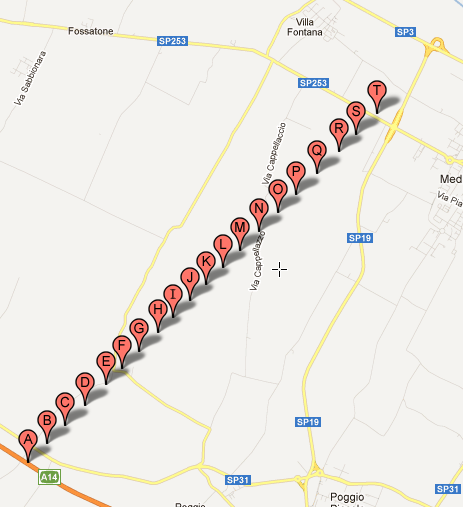
\includegraphics[width=3.4in]{imgs/punti_mappa.png}
	\caption{Fake positions used for the experiment}
	\label{fig:positions_experiment}
	\end{figure}

We tried our application with the following setting:
\begin{itemize}
	\item 3 Android devices;
	\item a set of fake position distributed on a straight line, each at a random distance between $275$ and $325$ meters from the following. In figure \ref{fig:positions_experiment} a graphical representation can be seen. They covers approximately $8$ kilometers;
\end{itemize}

